\documentclass[aspectratio=43]{beamer}
\usepackage[utf8]{inputenc}
\usepackage{polski}
% \usepackage[polish]{babel}
\usepackage[T1]{fontenc}
\usepackage{tikz}
\usepackage{tikzducks}
% \usetikzlibrary{decorations.pathmorphing}
\usepackage{multimedia}
\usepackage{graphicx}
\usepackage[justification=centering]{caption}
\usepackage{textcomp}
\usepackage{appendixnumberbeamer}
\usepackage{qrcode}
% \usepackage[natbib, language=polish, sorting=none]{biblatex}
% \addbibresource{lio.bib}
\usepackage{hyperref}
%\usepackage[width=\textwidth]{animate}
%\usepackage{chemformula}
\usepackage{sidecap}
\usepackage{multirow}
\usepackage{multicol}
\usepackage{rotating}
\usepackage{anyfontsize} % change font size for semposiwko

\usepackage{physics}
\usepackage{array}
\usepackage{booktabs}
\usepackage{transparent}
\usepackage{siunitx}
% \usepackage[rightcaption]{sidecap}
\usepackage{eso-pic}

\usepackage{listings}
\lstset{
basicstyle=\small\ttfamily,
columns=flexible,
breaklines=true
}

% \usepackage{emoji}
\usepackage{subcaption}


\usepackage[natbib, language=polish, sorting=none]{biblatex}
\addbibresource{lio.bib}
\renewcommand*{\bibfont}{\scriptsize}

\usefonttheme[onlymath]{serif}

\usetheme{Szeged}
\usecolortheme{whale}
\setbeamercolor{palette primary}{bg=violet!80!black,fg=white}
\setbeamercolor{palette secondary}{bg=violet!60!black,fg=white}
\setbeamercolor{palette tertiary}{bg=violet!40!black,fg=white}
\setbeamercolor{palette quaternary}{bg=violet!20!black,fg=white}
\setbeamercolor{structure}{fg=violet!60!black}
\setbeamertemplate{caption}{\insertcaption}
% \setbeamertemplate{headline}{
%   \begin{beamercolorbox}[wd=.9\paperwidth]{headline}
%     \vspace{1.5ex}
%     \insertsectionnavigationhorizontal
%     \vspace{1.5ex}
%   \end{beamercolorbox}
% }

\linespread{0.6}

\setbeamertemplate{background}%
{%
    \begin{tikzpicture}[remember picture,overlay]{\node[yshift=1.5cm,xshift=-2cm,opacity=0.1] at (current page.south east)
      {
      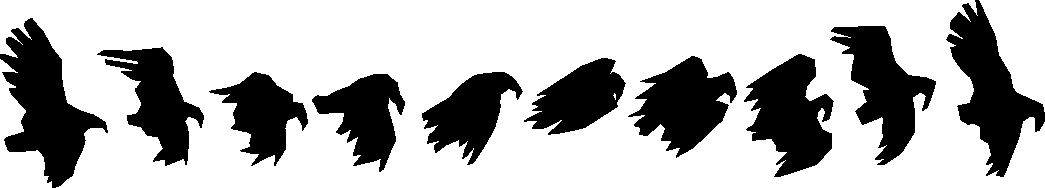
\includegraphics[scale=0.4, angle=20]{ptaki.pdf}
      }
      ;
    \node[yshift=1.0cm,xshift=0.6cm] (logopos) at (current page.south west) {{\begin{tikzpicture}\shuffleducks\duck[signpost=\insertframenumber, \randomhead,scale=.4]\end{tikzpicture}}};
    \pgfmathsetmacro{\progress}{360*(\insertframenumber)/(\inserttotalframenumber)};
    \draw[line width=0.2*3pt] ([xshift=0.55cm] logopos)  arc[radius=0.55cm, start angle=0, end angle=\progress];
    \fill ([shift={(\progress:0.55cm)}] logopos) circle(1pt);

    }
        \end{tikzpicture}
    
}

% \newcommand{\SeMPowisko}{%
% \large S\normalsize%
% \kern-.3em \lower.2ex\hbox{e}%
% \lower.2ex\hbox{\large M\normalsize}%
% \kern-.1em \raise.1ex\hbox{\large P\normalsize}%
% \kern-.3em \lower.2ex\hbox{o}%
% \kern-.2em \raise.2ex\hbox{w}%
% \lower.2ex\hbox{i}%
% s%
% \raise.2ex\hbox{k}%
% \kern-.3em \lower.2ex\hbox{o}%
% }

% \newcommand\Tikz{Ti\emph{k}Z}
% \definecolor{neworange}{RGB}{255,140,0}


\title{USG i endoskopia}
\subtitle{Aparatura medyczna w 30 sekund}
\author[M. Winiarski]{Mateusz ,,\(\blacksquare\)'' Winiarski}
\institute[Seminarium magisterskie]{biofizyka, FAIS, Uniwersytet Jagielloński}
\date[dzisiaj]{dzisiaj}

\begin{document}

\frame{\titlepage}


\section{USG}

\begin{frame}{Trochę historii}{}
    \begin{columns}
        \column{0.45\textwidth}
       \begin{figure}
\centering
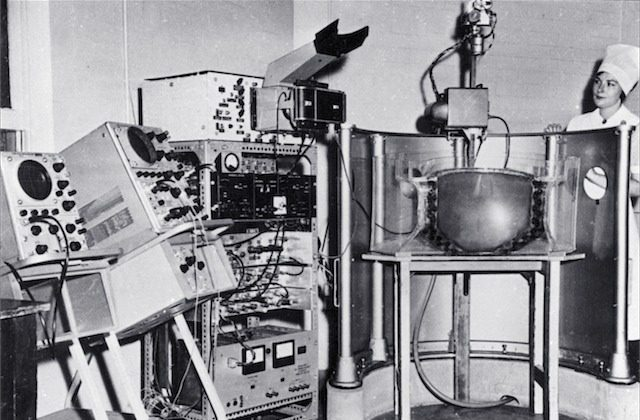
\includegraphics[width=\textwidth]{2025-03-05-01-34-57.png}
\caption{Aparat USG z lat 60.}
\end{figure}
\column{0.1\textwidth}
\vfill
{\LARGE \(\to\) }
\vfill
\column{0.45\textwidth}
\begin{figure}
\centering
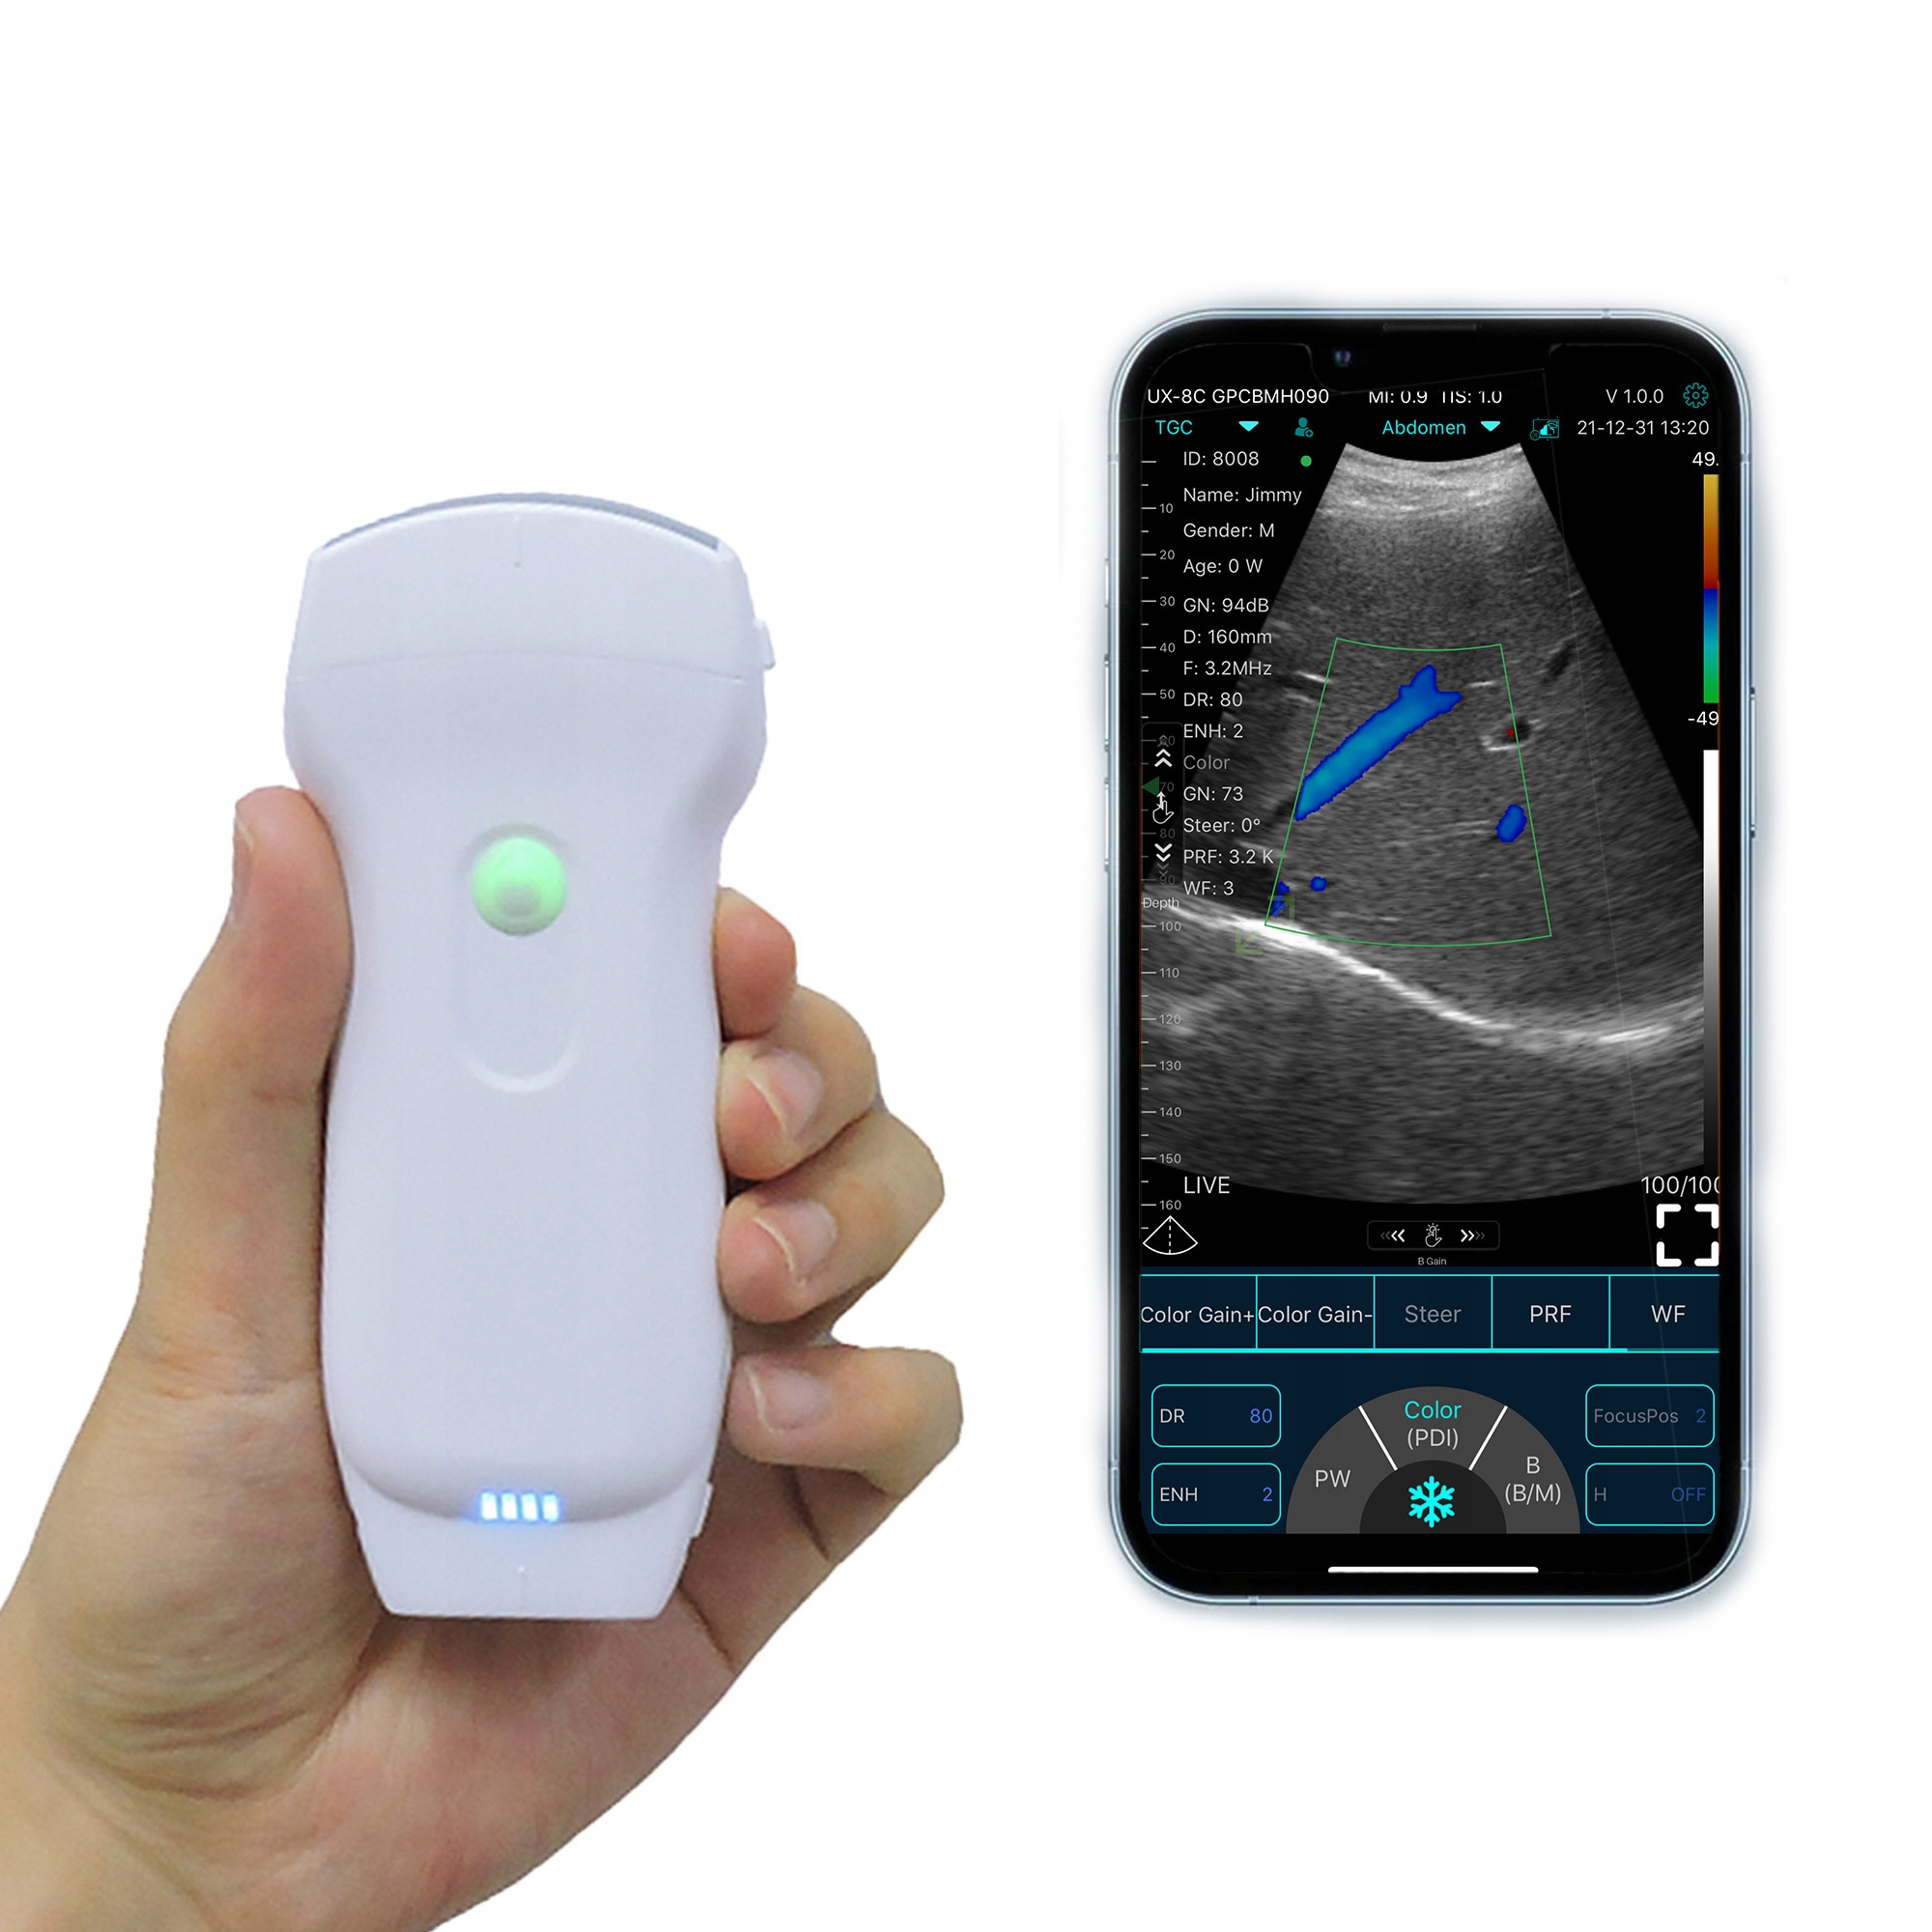
\includegraphics[width=\textwidth]{2025-03-05-01-48-54.png}
\caption{Współczesny miniaparat USG (na Allegro za 10k zł)}
\end{figure}
    \end{columns}
\end{frame} 
   
\begin{frame}{Trochę fizyki}{}
równanie falowe:
\[\nabla^2 p - \frac1{c^2} \frac{\partial^2 p}{\partial t^2}=0\]

prawo absorpcji:
\[I(x)=I_0 \exp(-\mu x)\] \[\mu=-\frac{1}{x} \frac1{\log e} \log \frac{I(x)}{I_0}\]

\[\mu=B\nu\]

\end{frame}

\begin{frame}{Tabelka}

    \begin{table}[h]
\centering
\caption{Wartości stałej B służącej do obliczenia współczynnika absorpcji fali akustycznej w wybranych tkankach oraz grubości warstwy połowicznego osłabienia [cm] dla trzech częstości}
\label{tab:absorpcja}
\begin{tabular}{|l|r|r|r|r|}
\hline
Tkanka & \(B\) & \multicolumn{3}{c|}{\(x_{1/2}\) \(I/I_0=0.5\)} \\
 & & 1 MHz & 2.25 MHz & 5 MHz \\ \hline
Krew & 0,087 & 34,60 & 7,69 & 4,32 \\ \hline
Tkanka tłuszczowa & 0,261 & 11,53 & 2,56 & 1,44 \\ \hline
Wątroba & 0,434 & 6,94 & 1,54 & 0,87 \\ \hline
Nerka & 0,478 & 6,30 & 1,40 & 0,79 \\ \hline
Mózg & 0,347 & 8,67 & 1,93 & 1,08 \\ \hline
Mięsień sercowy & 0,825 & 3,65 & 0,81 & 0,46 \\ \hline
Kość czaszki & 11,726 & 0,27 & 0,06 & 0,03 \\ \hline
\end{tabular}
\end{table}
    
\end{frame}

\begin{frame}{Trochę więcej fizyki}{}
    \begin{columns}
        \column{0.5\textwidth}
    \begin{figure}
    
        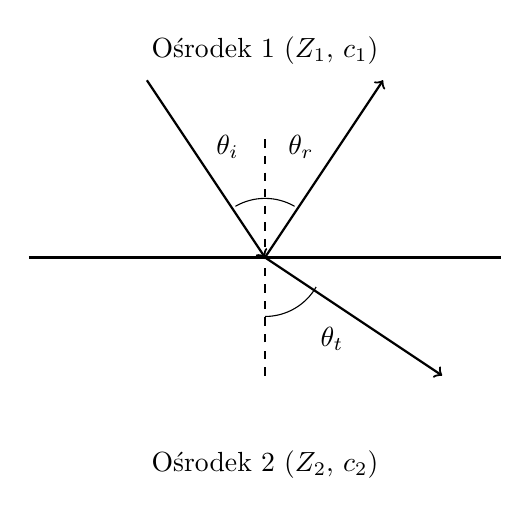
\begin{tikzpicture}[scale=0.75]

% Oznaczenia ośrodków
\node at (0, 3.5) {Ośrodek 1 ($Z_1$, $c_1$)};
\node at (0, -3.5) {Ośrodek 2 ($Z_2$, $c_2$)};

% Linia graniczna
\draw[thick] (-4, 0) -- (4, 0);

% Fala padająca
\draw[->, thick] (-2, 3) -- (0, 0) node[midway, above right] {$\theta_i$};
\draw[dashed] (-0, 2) -- (-0, 0);

% Fala odbita
\draw[->, thick] (0, 0) -- (2, 3) node[midway, above left] {$\theta_r$};
\draw[dashed] (-0, -2) -- (-0, 0);

% Fala załamana
\draw[->, thick] (0, 0) -- (3, -2) node[midway, below left] {$\theta_t$};
% \draw[dashed] (3, -2) -- (3, 0);

% Oznaczenia kątów
\draw (-0, 1) arc (90:120:1) node[midway, left] {};
\draw (-0, 1) arc (90:60:1) node[midway, left] {};
\draw (0, -1) arc (270:330:1) node[midway, right] {};

\end{tikzpicture}
    \end{figure}
    \column{0.5\textwidth}
    \[\frac{I_r}{I_i}+\frac{I_t}{I_i}=R+T=1\]
    \[R=\left(\frac{Z_2 \cos\theta_i-Z_1 \cos\theta_t}{Z_2 \cos\theta_i+Z_1\cos\theta_t}\right)^2\]
\end{columns}
\end{frame}

\begin{frame}{Trochę więcej liczb}{}
    \begin{table}[h]
\centering
\caption{Wartości współczynnika odbicia (R) dla wybranych granic organów w ciele pacjenta obliczone dla zerowego kąta padania}
\label{tab:odbicie}
\begin{tabular}{|l|c|}
\hline
\textbf{Granica tkanek} & \textbf{R} \\ \hline
Mięsień–powietrze & 0,9991 \\ \hline
Mięsień–woda & 0,0050 \\ \hline
Mięsień–płuca & 0,5905 \\ \hline
Mięsień–krew & 0,0007 \\ \hline
Mięsień–wątroba & 0,0002 \\ \hline
Mięsień–nerka & 0,0006 \\ \hline
Mięsień–kość długa & 0,4171 \\ \hline
Tk. tłuszczowa–mięsień & 0,0108 \\ \hline
Tk. tłuszczowa–wątroba & 0,0079 \\ \hline
Tk. tłuszczowa–nerka & 0,0064 \\ \hline
Kość czaszki–mózg & 0,4946 \\ \hline
\end{tabular}
\end{table}
\end{frame}

\begin{frame}{Wytwarzanie i detekcja fal}{}
    \begin{figure}
        \centering
        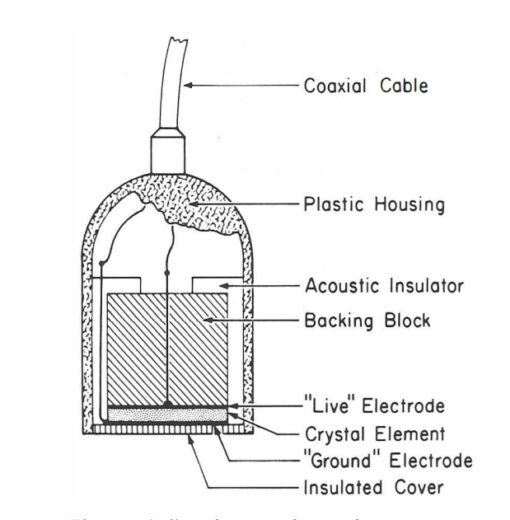
\includegraphics[width=0.5\textwidth]{2025-03-05-04-11-38.png}
        \caption{Schemat sondy USG}
    \end{figure}
\end{frame}

% \begin{frame}{Sonda USG}{}
    
% \end{frame}

\begin{frame}{Obrazowanie USG}{}
    \begin{itemize}
        \item prezentacja A (\emph{amplitude})
        \item prezentacja M (\emph{motion})
        \item prezentacja B (\emph{brightness})
    \end{itemize}

\begin{figure}
\centering
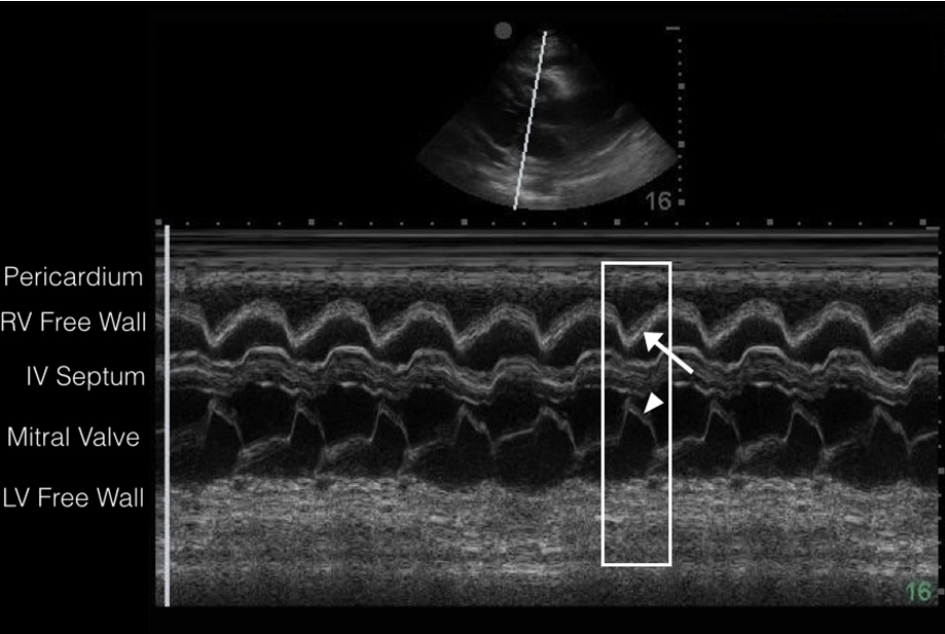
\includegraphics[width=0.65\textwidth]{2025-03-05-02-13-28.png}
\caption{{\scriptsize Obrazowanie w tamponadzie serca ukazujące zapadanie się wolnej ściany prawej komory (przemieszczanie się w kierunku przegrody międzykomorowej [strzałka]) podczas gdy zastawka mitralna jest otwarta [groty strzałki].}}
\end{figure}

\end{frame}

\begin{frame}{USG dopplerowskie}{}
    \[\nu_R=\nu_0\frac{c-v\cos\theta}{c}\]
    \begin{figure} \centering
    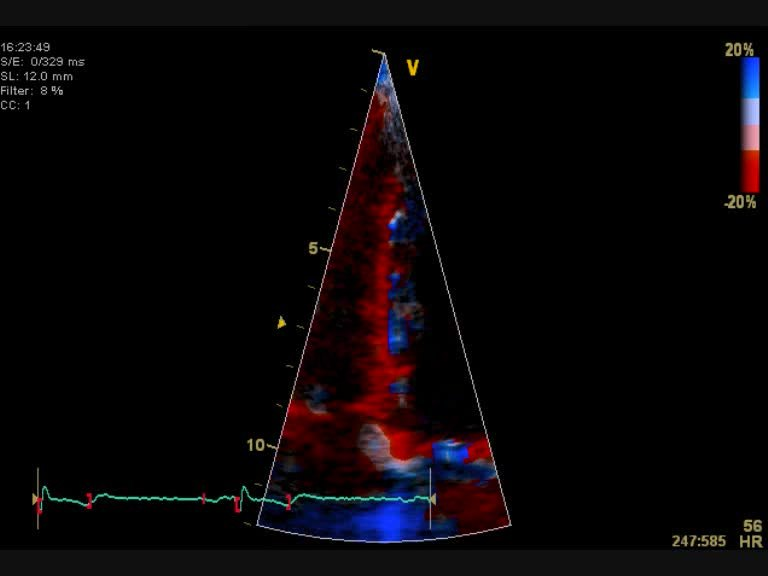
\includegraphics[width=0.65\textwidth]{2025-03-05-00-53-18.png}
    \caption{USG dopplerowskie przegrody międzykomorowej}
    \end{figure}
\end{frame}

\section{Endoskopia}


\begin{frame}{Endoskopia: historia}{}
        \begin{columns}
        \column{0.45\textwidth}
       \begin{figure}
\centering
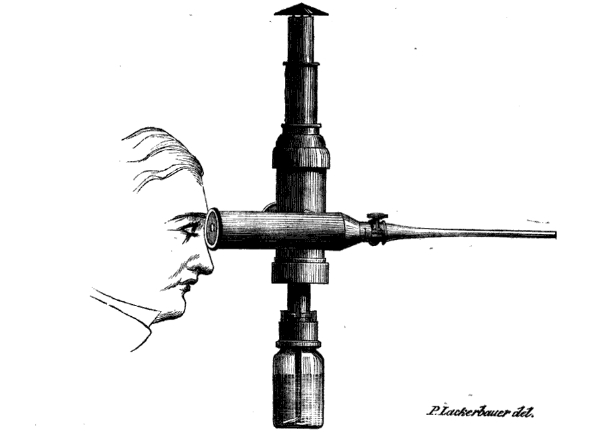
\includegraphics[width=\textwidth]{2025-03-05-03-18-44.png}
\caption{\emph{Lichtleiter} Philippa Bozziniego z 1806}
\end{figure}
\column{0.1\textwidth}
\vfill
{\LARGE \(\to\) }
\vfill
\column{0.45\textwidth}
\begin{figure}
\centering
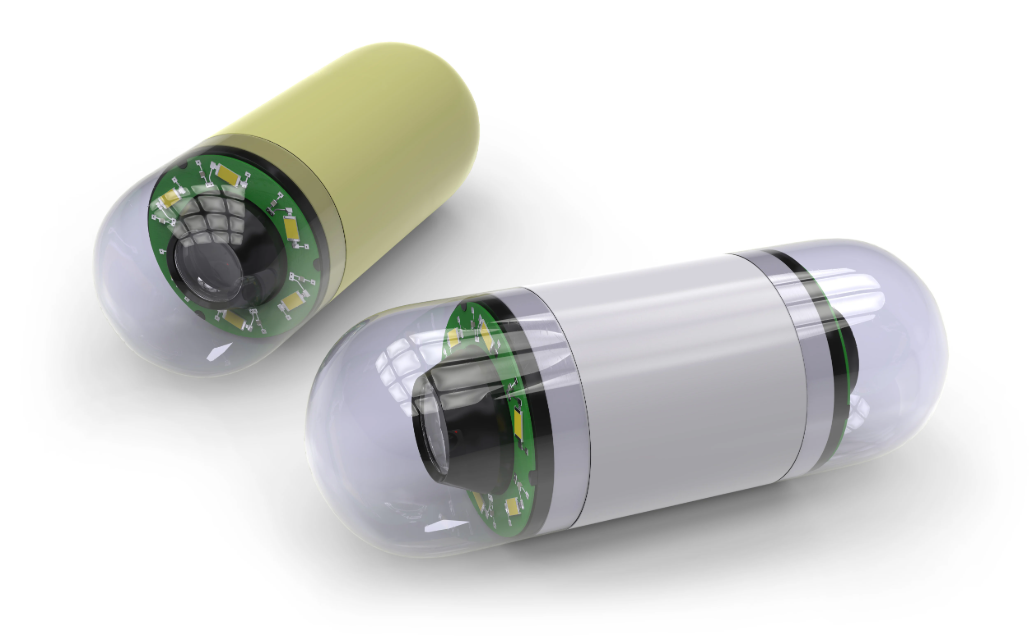
\includegraphics[width=\textwidth]{2025-03-05-03-20-33.png}
\caption{Endoskopy kapsułkowe}
\end{figure}
    \end{columns}
\end{frame}

\begin{frame}{Eksperyment}{}
    \begin{figure}
    \centering
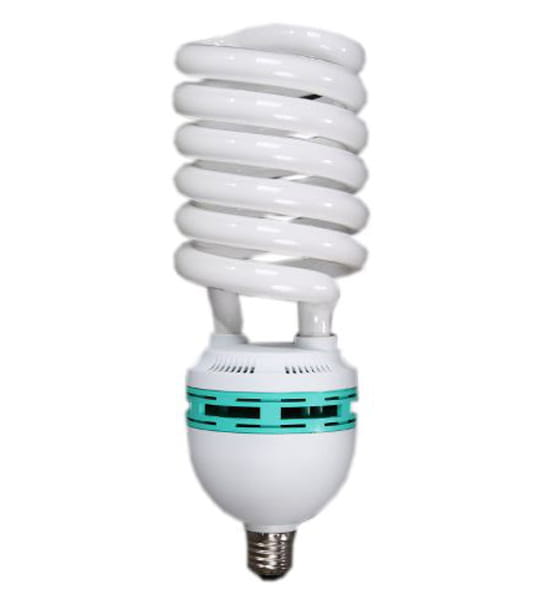
\includegraphics[width=0.5\textwidth]{2025-03-04-23-53-59.png}
\end{figure}
\nocite{LectureA,Blicharska_Hrynkiewicz_Rokita_2000,Hecht_2017,Kiesslich_Goetz_Hoffman_Galle_2011,Nakamura_Terano_2008,Zeng_2012}

\end{frame}

\begin{frame}{Światłowód}{}
    \[\theta_i'>\theta_c=\sin^{-1}\frac{n_2}{n_1}\]
    \[NA=\sqrt{n_1^2-n_2^2}=n_0\sin\theta_{max}\]
    \begin{figure}
        \centering
        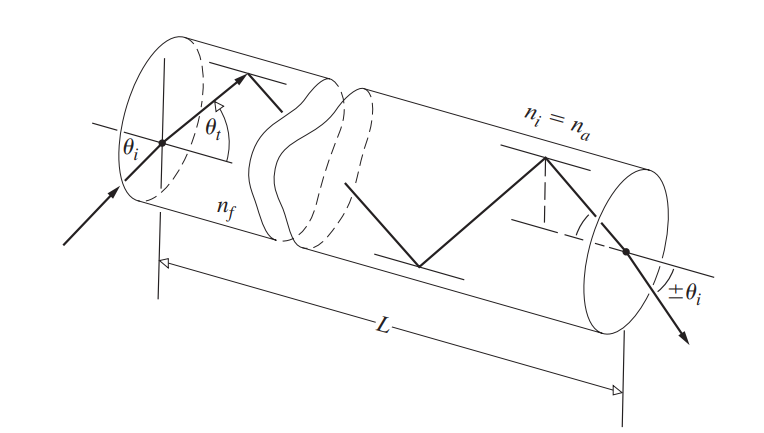
\includegraphics[width=0.8\textwidth]{2025-03-05-03-11-38.png}
    \end{figure}
\end{frame}

\begin{frame}{Endoskop sztywny i kapsułka endoskopowa}
    \begin{columns}
    \column{0.5\textwidth}
        \begin{figure}
            \centering
            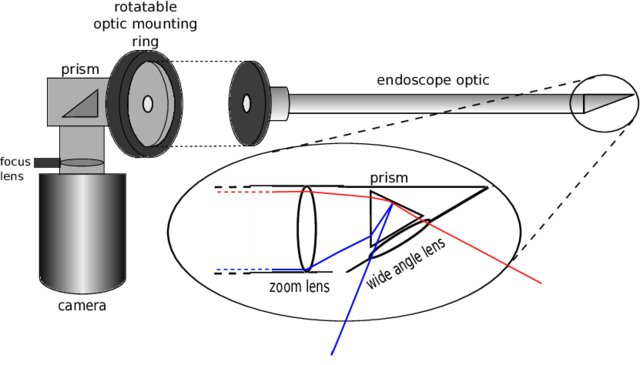
\includegraphics[width=\linewidth]{2025-03-05-09-24-39.png}
        \end{figure}

    \column{0.5\textwidth}

        \begin{figure}
            \centering
            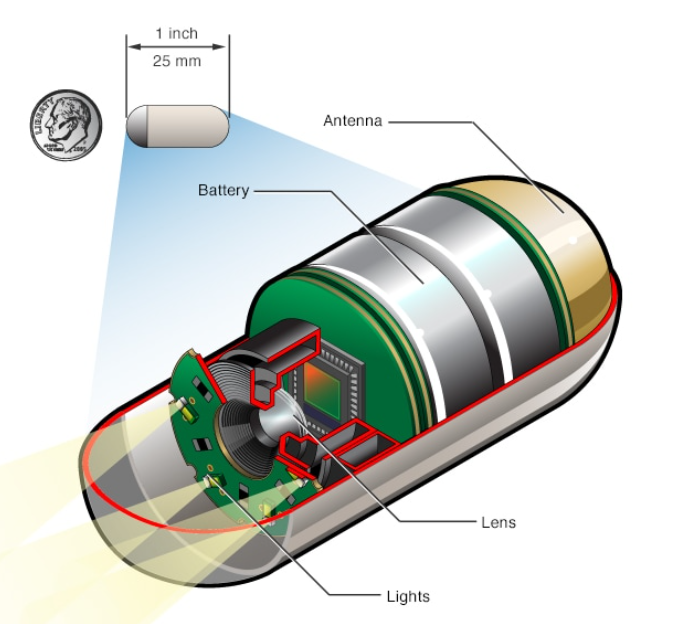
\includegraphics[width=\linewidth]{2025-03-05-10-02-05.png}
        \end{figure}

    \end{columns}
\end{frame}



\begin{frame}{Zastosowania}{}
    \begin{multicols}{3}
    \begin{itemize}
\item eso\-phago\-gastro\-duodeno\-scopy
\item enteroscopy
\item colonoscopy
\item sigmoidoscopy
\item magnification endoscopy
\item duodenoscope-assisted cholangiopancreatoscopy
\item intraoperative cholangioscopy
\item rectoscopy
\item anoscopy
% \item proctoscopy
% The respiratory tract
\item rhinoscopy
\item laryngoscopy
\item bronchoscopy
\item otoscopy
\item cystoscopy
\item ureteroscopy
\item gynoscopy
\item colposcopy
\item hysteroscopy
\item falloposcopy
% \item through a small incision:
\item laparoscopy
\item arthroscopy
\item thoracoscopy
\item mediastinoscopy
    \end{itemize}
\end{multicols}
\end{frame}

\begin{frame}{}
    \begin{columns}
        \column{0.32\textwidth}
        \begin{figure}
            \centering
            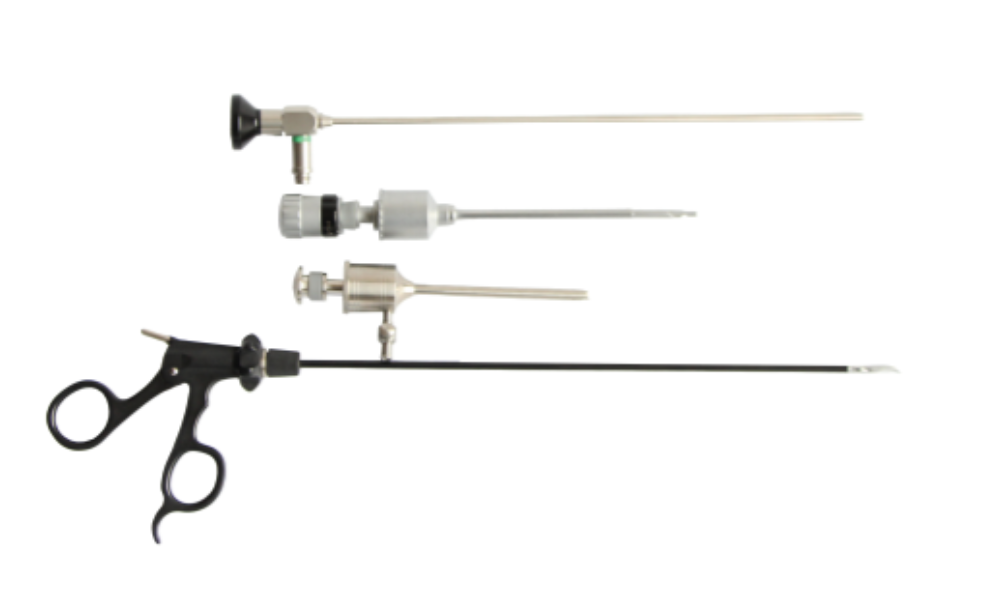
\includegraphics[width=\linewidth]{2025-03-05-09-32-38.png}
            \caption{endoskop sztywny}
        \end{figure}
        \column{0.32\textwidth}
        \begin{figure}
            \centering
            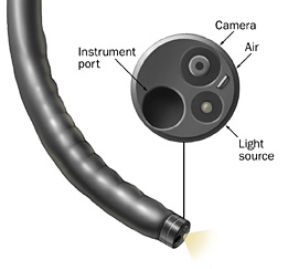
\includegraphics[width=\linewidth]{2025-03-05-13-03-37.png}
            \caption{endoskop giętki}
        \end{figure}
        \column{0.32\textwidth}
        \begin{figure}
            \centering
            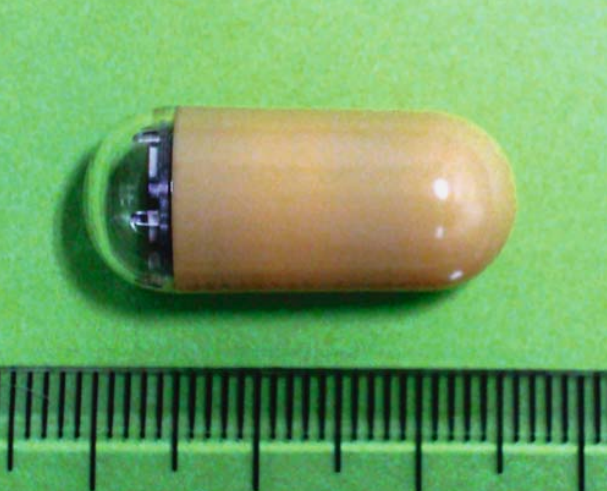
\includegraphics[width=\linewidth]{2025-03-05-09-54-45.png}
            \caption{kapsułka endoskopowa}
        \end{figure}
    \end{columns}
\end{frame}


\begin{frame}{}
    \begin{columns}
        \column{0.32\textwidth}
        \begin{figure}
            \centering
            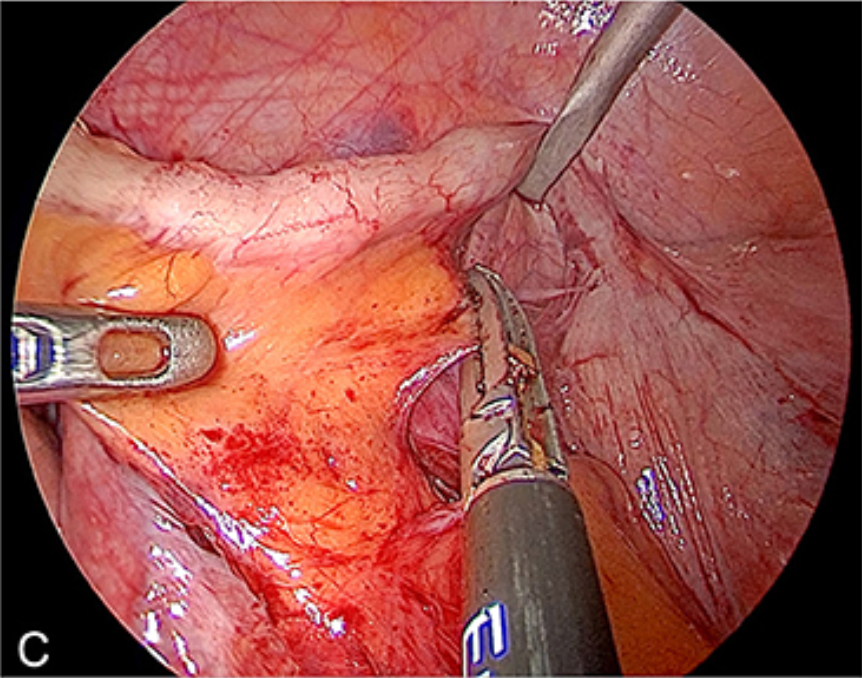
\includegraphics[width=\linewidth]{2025-03-05-09-36-03.png}
            \caption{laparoskopowe wycięcie wyrostka}
        \end{figure}
        \column{0.32\textwidth}
        \begin{figure}
            \centering
            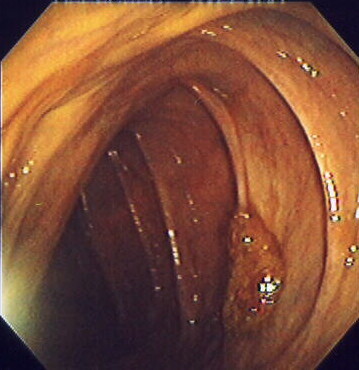
\includegraphics[width=\linewidth]{2025-03-05-13-54-25.png}
            \caption{kolonoskopia}
        \end{figure}
        \column{0.32\textwidth}
        \begin{figure}
            \centering
            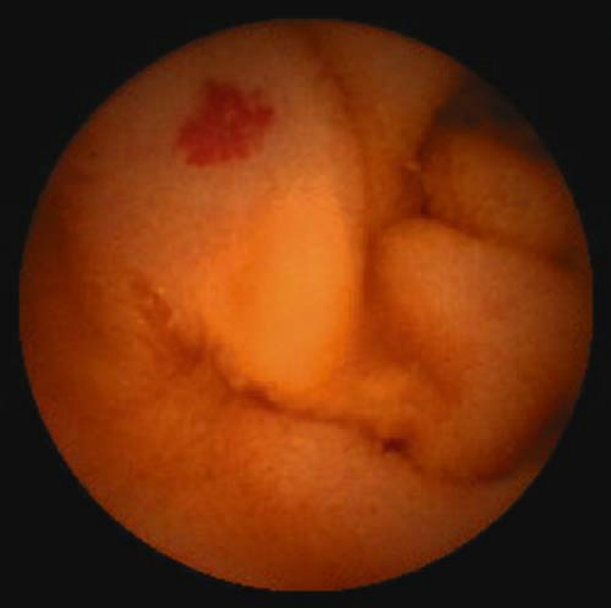
\includegraphics[width=\linewidth]{2025-03-05-09-55-52.png}
            \caption{enteroskopia jelita czczego}
        \end{figure}
    \end{columns}
\end{frame}

\begin{frame}{Inne zastosowania}
    \begin{columns}
    \column{0.5\textwidth}
    \begin{figure}
        \centering
        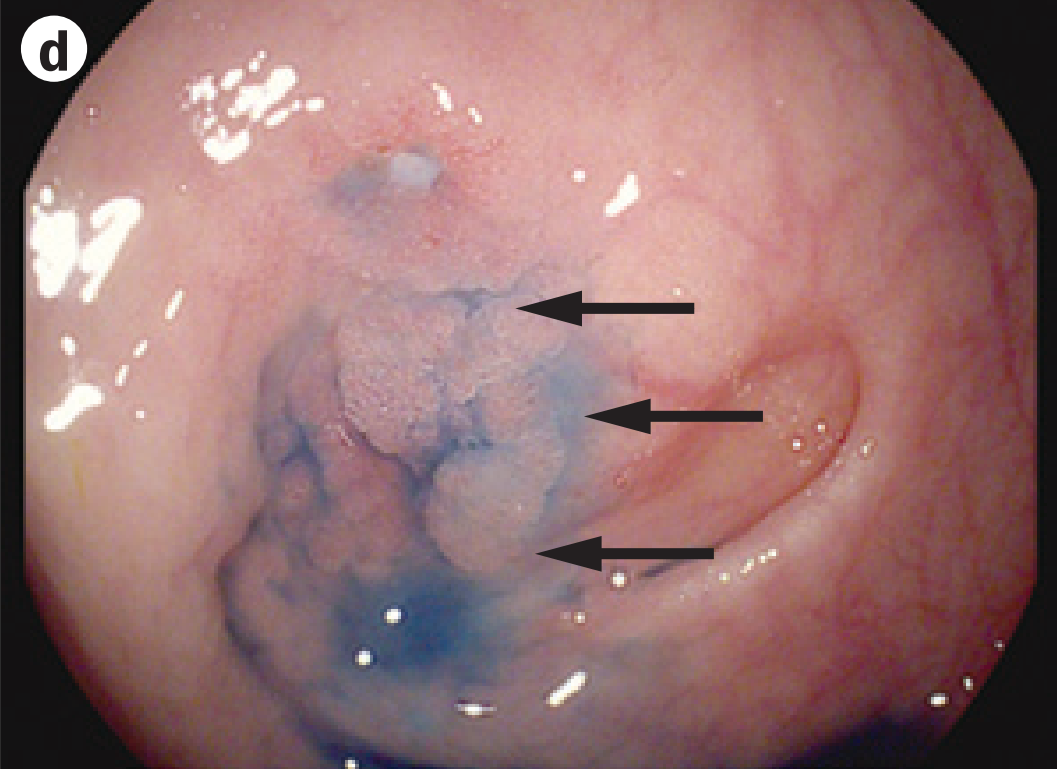
\includegraphics[width=\textwidth]{2025-03-05-11-26-29.png}
        \caption{chromoendoskopia używająca błękitu metylenowego}
    \end{figure}
    \column{0.5\textwidth}
    \begin{figure}
        \centering
        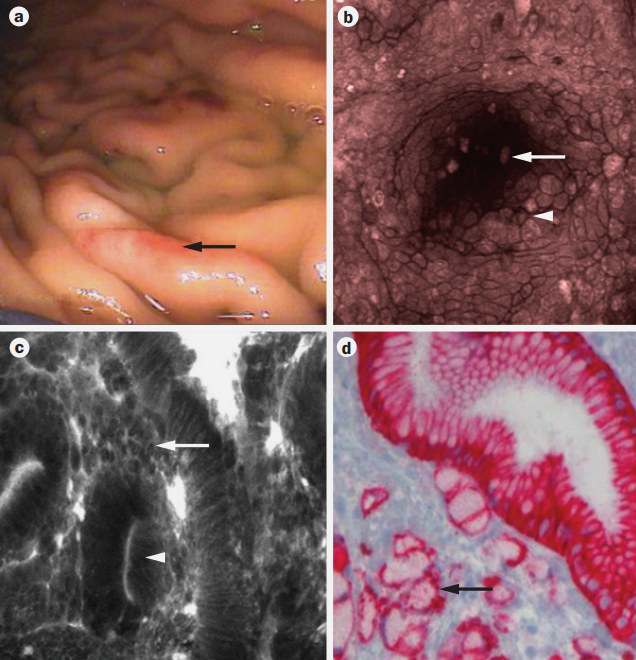
\includegraphics[width=\textwidth]{2025-03-05-12-11-38.png}
        \caption{endomikroskopia (b,c) vs histologia (d)}
    \end{figure}
    \end{columns}
\end{frame}





\section{}

\begin{frame}{Bibliografia}{}
    \printbibliography[heading=none]
\end{frame}

\begin{frame}{}{}
    \vspace{-1.5cm}
\begin{figure}
\centering
    \begin{tikzpicture}
      \duck[parrot, body=gray!30!yellow, head=gray!30!yellow, bill=red, torch=gray!70!brown, tshirt=blue!40!black, ribbon=gray, bowtie=blue!50!white, crazyhair=black]
      %\addwater{blue!50!cyan}
      \fill[cyan!20!white] (-1.4,1.8) ellipse (1.8 and 0.5);
  \fill[cyan!20!white] (-0.2,1.54) -- (0.2,1.35) -- (0.0,1.6) -- cycle;
	\node at (-1.4,1.8) {dziękuję za uwagę};
    \end{tikzpicture}
    \end{figure}


    
    \begin{figure}
    \centering
    \qrcode[height=0.3\textwidth]{https://github.com/falcotinnunculus/przezrocza/blob/wladca/sb2/main.pdf}\\
    {\tiny \url{https://github.com/falcotinnunculus/przezrocza/blob/wladca/sb2/main.pdf}}

    \end{figure}
\vspace{-4.15cm}
\transparent{0.5}
    \begin{figure}
        \centering
        % 
\includegraphics[height=0.3\linewidth]{jez.png}
        % \caption{Caption}
        % \label{fig:enter-label}
    \end{figure}
\end{frame}

\appendix

\begin{frame}{Źródła obrazów}{}
    \scriptsize
    \begin{itemize}
        % \item
    \item \url{https://cdn2.hubspot.net/hubfs/2027031/capsule endoscopy.jpeg}
    \item \url{https://www.sciencedirect.com/science/article/abs/pii/S0736467915006812}
    \item \url{https://commons.wikimedia.org/wiki/File:Endoscope_-_Position_durant_l'application.jpg}
    \item \url{https://www.asum.com.au/wp-content/uploads/2015/08/100_UI0024-e1592443996756.jpg}
    \item \url{https://allegro.pl/oferta/przenosne-bezprzewodowe-usg-ultrasonograf-color-doppler-linia-convex-cardio-12083641435}
    \item \url{https://www.researchgate.net/publication/200058404_Dynamic_Distortion_Correction_for_Endoscopy_Systems_with_Exchangeable_Optics/}
    \item \url{https://www.manomedical.com/en/endoscopy/veterinary-video-laparoscope}
    \item \url{https://www.mayoclinic.org/tests-procedures/capsule-endoscopy/about/pac-20393366}
    \item \url{https://safesurgery.com.au/services/colonoscopy-gastroscopy/}
    \item \url{https://commons.wikimedia.org/wiki/File:Endomucosal_resection_1.jpg}
    \end{itemize}
\end{frame}


\end{document}